% !TEX program = XeLaTeX
% !BIB program = bibtex
\documentclass[12pt, a4paper, oneside]{book}
\usepackage{amsmath}
\usepackage{amssymb}
\usepackage{amsthm}
\usepackage{graphicx}
\usepackage{latexsym}
\usepackage{pslatex}
\usepackage{color}
\usepackage{cite}
\usepackage{indentfirst}
\usepackage{tocloft}
\usepackage{multirow}
\usepackage{fontspec}

% Times New Roman
\setromanfont[
BoldFont=Times New Roman Bold.ttf,
ItalicFont=Times New Roman Italic.ttf,
BoldItalicFont=Times New Roman Bold Italic.ttf,
]{Times New Roman.ttf}
%\setmainfont{Times New Roman}

% Centering Chapter
\usepackage{sectsty}
\chapterfont{\centering}

\pagestyle{myheadings}
\setlength{\parindent}{0.8in}

\usepackage[top=1.5in,bottom=1in,left=1.5in,right=1in]{geometry}

\theoremstyle{plain}
\newtheorem{thm}{Theorem}[chapter]
\newtheorem{lem}[thm]{Lemma}
\newtheorem{cor}[thm]{Corollary}
\newtheorem{prop}[thm]{Proposition}
\newtheorem{rem}[thm]{Remark}
\newtheorem{ex}[thm]{Example}
\newtheorem{de}[thm]{Definition}
\renewcommand{\proof}{\textbf{Proof.}}

\numberwithin{equation}{chapter} \DeclareMathOperator{\Var}{var}
\DeclareMathOperator{\Ima}{Im}

\usepackage{float}
%\usepackage[skip=2pt,font=footnotesize]{caption}

\usepackage{graphics,graphicx}
\usepackage{calc}
\usepackage{tikz}
\usetikzlibrary{decorations.markings}
\tikzstyle{vertex}=[circle, draw, inner sep=2pt, minimum size=4pt]
\newcommand{\vertex}{\node[vertex]}
\newcounter{Angle}

\renewcommand{\baselinestretch}{1.5}

\newcommand*{\QEDA}{\hfill\ensuremath{\large{\lozenge}}}
\newcommand*{\QEDAa}{\hfill\ensuremath{\square}}

\renewcommand{\bibname}{\centerline{\Large REFERENCES}}

\usepackage{tocloft}
\renewcommand{\contentsname}{\hfill\bfseries\Large TABLE OF CONTENTS \hfill}
\renewcommand{\cftaftertoctitle}{\hfill}

\renewcommand{\listtablename}{\hfill\bfseries\Large LIST OF TABLES}
\renewcommand{\cftafterloftitle}{\hfill}

\renewcommand{\listfigurename}{\hfill\bfseries\Large LIST OF FIGURES}
\renewcommand{\cftafterloftitle}{\hfill}



\renewcommand{\cftchapleader}{\cftdotfill{\cftdotsep}}
\renewcommand{\cftsecleader}{\cftdotfill{\cftdotsep}}
\renewcommand{\cftsubsecleader}{\cftdotfill{\cftdotsep}}
\renewcommand{\contentsname}{Mục lục}
\renewcommand{\chaptername}{Chương}

\usepackage{titlesec}
\titleformat{\chapter}[block]{\centering\normalfont\huge\bfseries}{\chaptername~\thechapter.}{0.5em}{}

\graphicspath{{assets/}}

\usepackage{listings}

\usepackage[colorlinks=true, linkcolor=blue]{hyperref}

\begin{document}
% --- Trang bìa ---
\thispagestyle{empty}
\begin{center}
    \begin{figure}[h!]
    \centering
    
\includegraphics[width = 7.0cm]{HCMCOU_Logo.png}
    \end{figure}

    {\fontsize{30pt}{25pt}\selectfont\bfseries
    FACE DETECTION WITH RETINAFACE\par}
    \vspace{2.0cm} 

    {\fontsize{20pt}{25pt}\selectfont\bfseries
    ĐỒ ÁN MÔN HỌC\par}
    \vspace{0.25cm}
    {\fontsize{15pt}{25pt}\selectfont\bfseries
    Môn: Máy học\par}
    \vspace{5.0cm}
    
    {\fontsize{20pt}{15pt}\selectfont\bfseries
    TP. HỒ CHÍ MINH, 2026}
\end{center}

\newpage
\thispagestyle{empty}
\begin{center}
    \begin{figure}[h!]
    \centering
    
\includegraphics[width = 7.0cm]{HCMCOU_Logo.png}
    \end{figure}

    {\fontsize{25pt}{20pt}\selectfont\bfseries NHÓM 6\par}
    \vspace{1.5cm}
    {\large \textbf{THÀNH VIÊN}}\\
    \vspace{0.3cm}
    {\large
    \begin{tabular}{r c l}
        \textbf{2351010176} & \textbf{-} & \textbf{Phạm Minh Quân} \\
        \textbf{2351010238} & \textbf{-} & \textbf{Lê Khắc Tùng} \\
        \textbf{2351010227} & \textbf{-} & \textbf{Phạm Quý Trưởng} \\
        \textbf{2351010242} & \textbf{-} & \textbf{Nguyễn Bảo Việt} \\
        \textbf{2351010228} & \textbf{-} & \textbf{Hoàng Việt Tuấn} \\
    \end{tabular}}
    \vspace{2.0cm}

    {\fontsize{17pt}{15pt}\selectfont\bfseries
    Giáo viên hướng dẫn: LÊ VIẾT TUẤN}
    \vspace{3.0cm}

    {\fontsize{20pt}{15pt}\selectfont\bfseries
    TP. HỒ CHÍ MINH, 2026}
\end{center}

% --- Mục lục ---
\newpage
\pagenumbering{roman} 
\tableofcontents
\newpage

% --- NỘI DUNG ---
\pagenumbering{arabic} 
\setcounter{page}{1}
\pagestyle{myheadings}

\chapter{Giới thiệu}
\section{Tổng quan paper: }
\begin{itemize}
    \item[--] Bài toán nhận diện khuôn mặt đã trở thành một trong những bài toán kinh điển trong lĩnh vực \textbf{AI for Computer Vision}
    \item[--] Mặc dù có những bước tiến vượt bậc trong việc phát hiện \textbf{uncontrolled face} -- phát hiện được những khuôn mặt trong những thách thức về không gian như ánh sáng, pose hay những góc khuất, việc định vị chính xác và hiệu quả khuôn mặt trong môi trường thực tế vẫn đang là thách thức lớn chưa được giải quyết triệt để. 
    \item[--] RetinaFace -- Single-stage face detector, được giới thiệu là một giải pháp mạnh mẽ trong việc phát hiện từng \textbf{pixel-wise} (điểm ảnh) trên nhiều tỉ lệ khuôn mặt khác nhau bằng cách tận dụng lợi thế của \textbf{extra-supervised} và \textbf{self-supervised multi-task learning}.
\end{itemize}

\subsection{Extra-supervised Learning -- Học có giám sát bổ sung:}
\begin{itemize}
    \item[--] Trong Supervised Learning, mô hình được huấn luyện dựa trên bộ dữ liệu có label.
    \item[--] Trong Extra-supervised Learning, ngoài label có sẵn, ta \textbf{cung cấp thêm} cho mô hình các \textbf{auxiliary labels (nhãn phụ trợ)} chi tiết hơn ở một khía cạnh khác so với label của tác vụ chính.
    \item[--] Mục đích:
    \begin{itemize}
        \item[+] Giảm Overfitting: Việc phải dự đoán đúng nhiều loại label cùng lúc giúp mô hình học được các đặc trưng tổng quát hơn, thay vì chỉ học vẹt một tác vụ duy nhất.
        \item[+] Giúp mô hình chú ý đến các chi tiết quan trọng của dữ liệu mà nếu chỉ sử dụng 1 label chính, mô hình có thể bỏ qua.
    \end{itemize}
\end{itemize}
\subsection{Self-supervised Multi-task Learning -- Học đa tác vụ tự giám sát:}
\begin{itemize}
    \item[--] \textbf{Self-supervised learning (Học tự giám sát):} Là phương pháp học mà mô hình tự tạo ra label từ dữ liệu gốc mà không cần gán label thủ công.
    \item[--] \textbf{Multi-task learning (Học đa tác vụ):} Là phương pháp thiết kế một neurel network duy nhất để giải quyết nhiều bài toán khác nhau cùng một lúc (chia sẻ chung các layer trích xuất đặc trưng đầu vào).
    \item[--] \textbf{Self-supervised Multi-task Learning: } Là mô hình học song song nhiều tác vụ cùng một lúc, trong đó có ít nhất một tác vụ tự tạo ra nhãn từ input.
    \item[--] Mục đích:
    \begin{itemize}
        \item[+] Tận dụng tối đã dữ liệu chưa gán nhãn: Cho phép mô hình học các biểu diễn hình học, cấu trúc hoặc ngữ cảnh thông qua nhánh self-supervised, từ đó hỗ trợ tăng cường độ chính xác cho các nhánh học có giám sát khác.
    \end{itemize}     
\end{itemize}

\section{WIDER FACE Dataset:}
\begin{itemize}
    \item[--] RetinaFace sử dụng \textbf{WIDER FACE} dataset -- \textbf{Face Detection Benchmark} \cite{yang2016wider}.
    \item[--] Bộ dataset này chứa nhiều annotations khác nhau bao gồm: Occlusions (độ che khuất), poses, event categories, face bounding boxes...
    \item[--] WIDER FACE bao gồm 32,203 ảnh và 393,703 face bounding boxes với mức độ biến đổi cao về scale, poses, expression, occlusion và illumination.
    \item[--] WIDER FACE được chia thành 40\% training, 10\% validation và 50\% testing bằng cách \textbf{randomly sampling} (Lấy mẫu ngẫu nhiên) từ 61 scene categories.
    \item[--] Dựa vào tỷ lệ phát hiện của thuật toán EdgeBox, khuôn mặt được phân thành 3 levels: Easy, Medium và Hard Thông qua việc bổ sung dần các mẫu khó. 
    \item[--] \textbf{Extra Annotations.} Nhóm tác giả paper đã xác định được 5 cấp độ chất lượng hình ảnh khuôn mặt (levels of face image quality) và tiến hành gán nhãn thủ công, bổ sung 5 điểm mốc khuôn mặt (facial landmarks) bao gồm: tâm 2 mắt, chóp mũi và 2 khóe miệng. 
    \begin{figure}[h!]
        \centering
        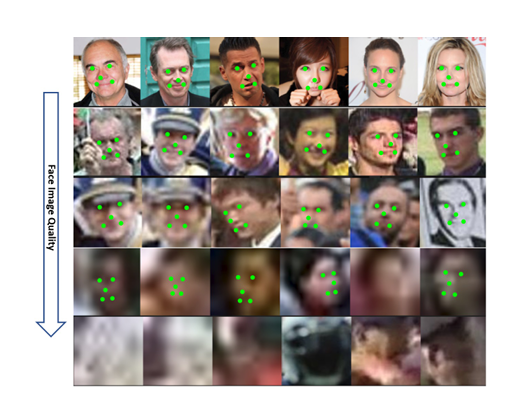
\includegraphics[width=0.8\textwidth]{extra_annotations.png}
        \caption{Các extra annotations của 5 facial landmarks}
    \end{figure}
    \item[--] Tổng cộng đã gán nhãn 84,600 faces trên training set và 18,500 faces trên validation set
\end{itemize}


\chapter{Metrics và Box trong Face Detection}
\section{Bounding Box:}
\begin{itemize}
    \item[--] Bounding box là phần khung bao quanh 1 object.
    \item[--] \textbf{Các chuẩn biểu diễn tọa độ phổ biến: }
        \item[+] Min max: $(x_{min}, y_{min}, x_{max}, y_{max})$   
        \item[+] Center-Size: $(x_{center}, y_{center}, width, height)$ 
    \vspace{0.2cm}
    \begin{figure}[h!]
        \centering
        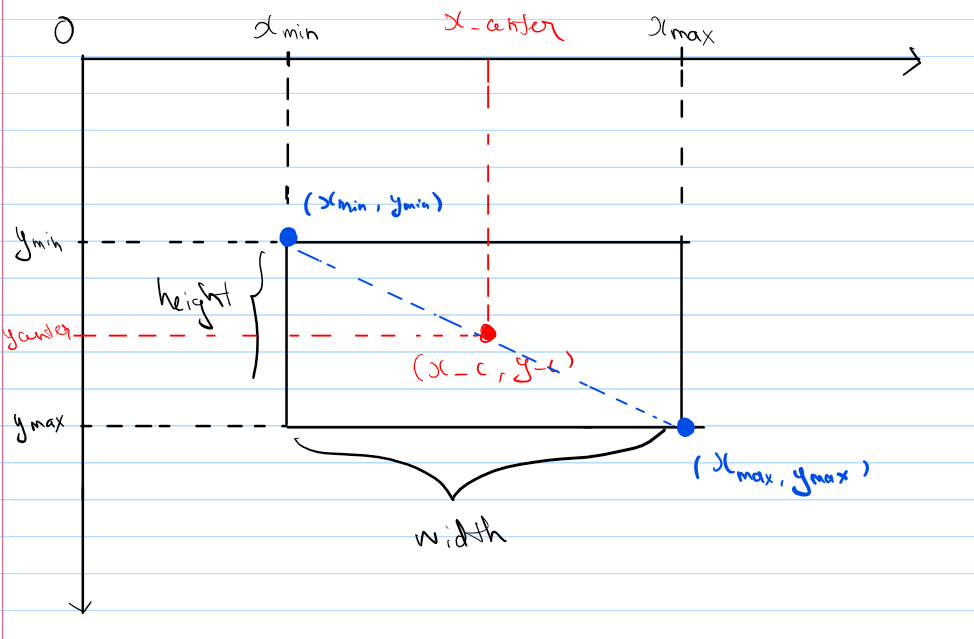
\includegraphics[width=0.8\textwidth]{coordinate.png}
        \caption{Hệ trục tọa độ của các điểm trên}
    \end{figure}
\end{itemize}


\section{WIDERFACE Annotations:}
\begin{itemize}
    \item[--] \textbf{Cấu trúc annotations} trong label.txt mà paper cung cấp:
        \item[+] File name
        \item[+] Number of bounding Box
        \item[+] \(x_1\), \(y_1\), w, h, blur, expression, illumination, invalid, occlusion, pose
\end{itemize}

\section{Jaccard:}
\begin{itemize}
    \item[--] \textbf{Jaccard Index (Hệ số tương đồng Jaccard)} -- là một con số dùng để đo lường mức độ tương đồng giữa hai tập hợp dữ liệu trong xác suất thống kê (statistic)
    \[J(A,B) = \frac{|A \cap B|}{|A \cup B|} = \frac{|A \cap B|}{|A| + |B| - |A \cap B|}\]
\end{itemize}

\section{Intersection over Union (IoU):}
\begin{itemize}
    \item[--] \textbf{IoU} là một metric dùng để đánh giá mức độ trùng lấp (overlap) giữa 2 bounding boxes.
    \item[--] Công thức tổng quát:
    \[\textbf{IoU} = \frac{\textbf{Area of Intersection}}{\textbf{Area of Union}}\] 
    
    \begin{figure}[H]
        \centering
        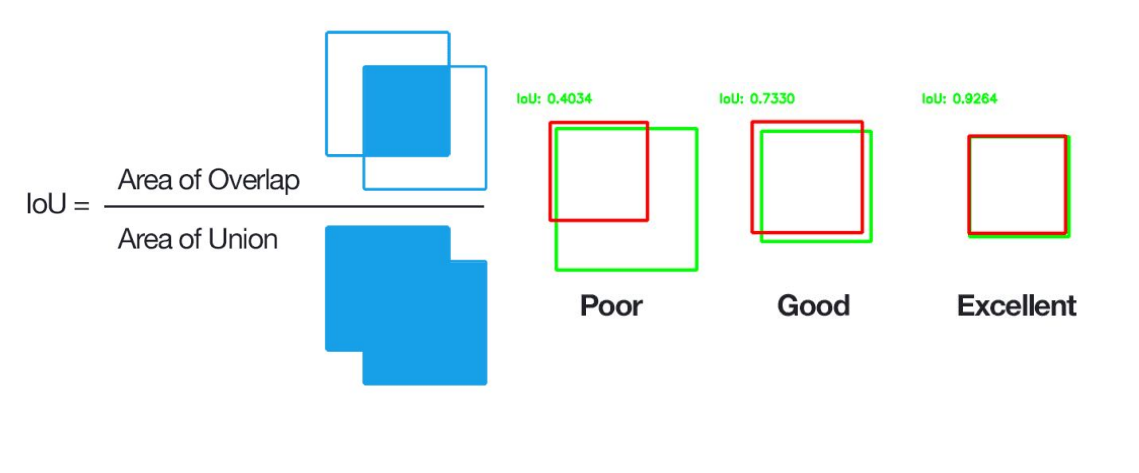
\includegraphics[width=0.8\textwidth]{IoU.png}
        \caption{Minh họa IoU}
    \end{figure}

    \subitem \textbf{Intersection:} Phần giao giữa hai bounding boxes
    \subitem \textbf{Union:} Phần hợp giữa hai bounding boxes
    \item[--] Hai bounding boxes càng overlap nhau, IoU càng \textbf{gần 1}, độ chính xác càng cao, object được detect càng tốt.
    \item[--] Hai bounding boxes càng lệch nhau, IoU càng \textbf{gần 0}, độ chính xác càng giảm, object dectect sai 
\end{itemize}

\section{Average Precision và Mean Average Precision:}
\subsection{Average Precision (AP):}
\begin{itemize}
    \item[--] AP dùng để đo độ chính xác của mô hình cho một class duy nhất.
    \item[--] Cách tính:
    \begin{enumerate}
        \item[+] Liệt kê tất cả các bounding boxes mà mô hình dự đoán được, sắp xếp giảm dần dựa vào \textbf{confidence score}
        \item[+] So sánh với ground truth bằng IoU qua threshold (Ngưỡng), thường là 0.5.
        \begin{itemize}
            \item[.] \textbf{True Positive (TP):} Dự đoán có IoU \(\ge\) threshold với Ground Truth
            \item[.] \textbf{False Positive (FP):} Dự đoán có IoU < threshold với Ground Truth
            \item[.] \textbf{False Negative {FN}:} Grouth truth mà mô hình bỏ lỡ (không detect được)
        \end{itemize}
        \item[+] Tính Precision và Recall:
        \[Precision = \frac{TP}{TP + FP}\ \quad ; \quad Recall = \frac{TP}{TP + FN}\]
        \item[+] Vẽ Precision-Recall Curve:
        \begin{figure}[H]
            \centering
            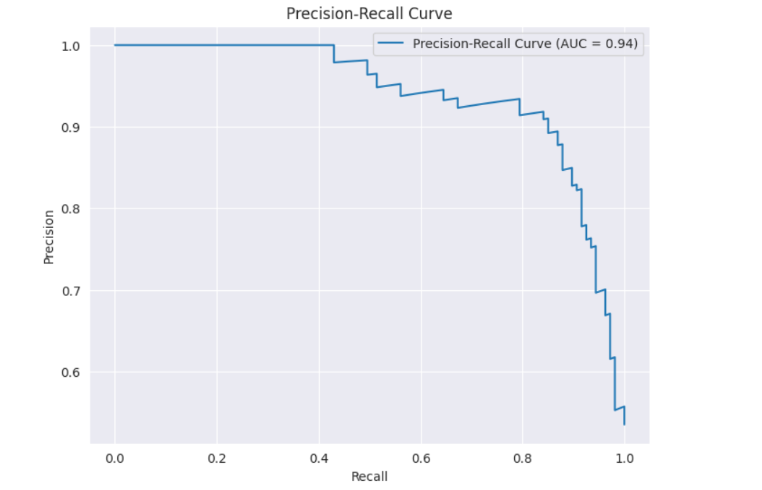
\includegraphics[width=0.7\textwidth]{precision_recall_curve.png}
            \caption{Minh họa Precision-Recall Curve}
        \end{figure}
        \item[+] AP = diện tích dưới đường Precision-Recall (Area under the precision-recall curve AUC-PR)
        \item[+] Công thức tổng quát:
        \[AUCPR = \int_{0}^1 P(R) \, dR\]
        \begin{itemize}
            \item[.] \(P(R)\): precision tại recall R
        \end{itemize} 
        \item[+] Công thức rời rạc:
        \[AUCPR = \sum_{n} (R_n - R_{n-1}) P_n\]
        \begin{itemize}
            \item[.] \(P_n\): Precision tại điểm n
            \item[.] \(R_n\): Recall tại điểm n
            \item[.] \(R_n - R_{n-1}\): Độ tăng recall (\(R_n\) và \(R_{n-1}\) là các mức Recall kế tiếp nhau sau khi đã sắp xếp theo Confidence Score)
        \end{itemize}
            
    \end{enumerate}    
\end{itemize}
\subsection{Mean Average Precision (mAP):}
\begin{itemize}
    \item[--] mAP là trung bình giá trị AP của tất cả classes.
    \[mAP = \frac{1}{N}\sum_{i=1}^{N}A{P_i}\]
    \begin{itemize}
        \item[+] \(N\): Số lượng classes.
        \item[+] \(A{P_i}\): giá trị AP tại class thứ i.
    \end{itemize}

\end{itemize}

\chapter{Related works}
\section{Image Pyramid và Feature Pyramid:}
Image Pyramid và Feature Pyramid là hai phương pháp được sử dụng để giải quyết thách thức về sự thay đổi tỷ lệ (scale) kích thước khuôn mặt.
\subsection{Image Pyramid}
\begin{itemize}
    \item[--] Mô hình dựa trên cơ chế sliding-windows, trong đó classifier sẽ được quét qua một lưới hình ảnh dày đặc (dense image grid)
\end{itemize}
\subsection{Feature Pyramid}
\begin{itemize}
    \item[--] Mô hình được xây dựng dựa trên \textbf{Image Pyramid}, kết hợp giữa sliding-anchor (cơ chế mỏ neo trượt) trên multi-scale feature maps đã thống trị \textbf{(dominated)} trong lĩnh vực face detection.
\end{itemize}
\begin{figure}[H]
    \centering
    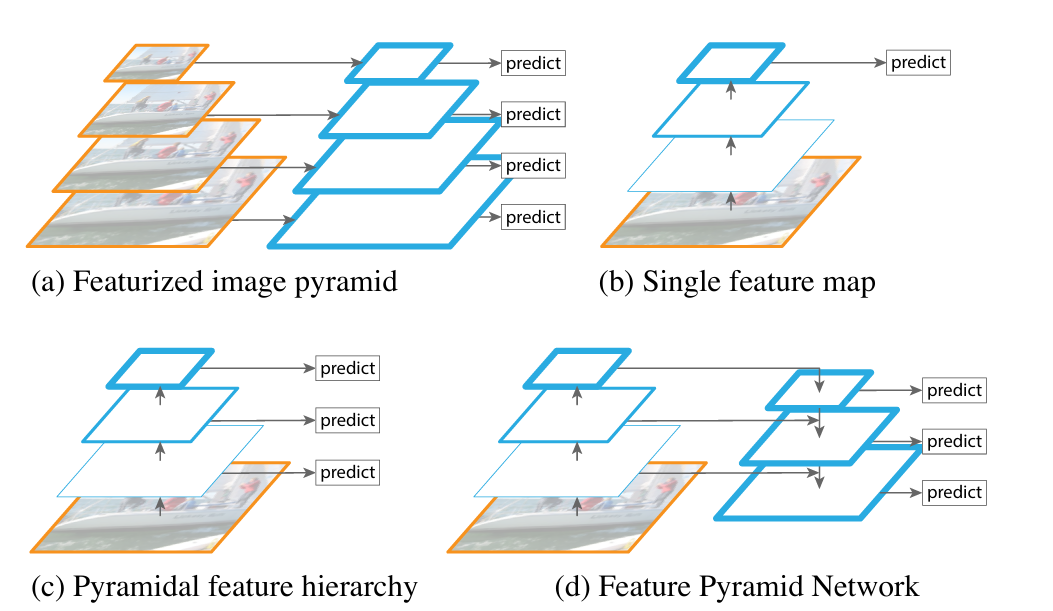
\includegraphics[width=1\textwidth]{pyramid.png}
    \caption{Minh họa Feature Pyramid được xây dựng dựa trên Image Pyramid}
\end{figure}

\section{Two-stage và Single-stage:}
\subsection{Two-stage:}
\begin{itemize}
    \item[--] \textbf{Giai đoạn 1 - Đề xuất vùng (Region Proposal Generation):} Sử dụng các thuật toán như Selective Search hoặc Region Proposal Network (RPN) trong các kiến trúc hiện đại (Faster R-CNN) để xác định các vùng ứng viên có khả năng chứa object.
    \item[--] \textbf{Giai đoạn 2 - Phân loại và Tinh chỉnh (Classification \& Regression):} Với mỗi Region Proposal, mô hình thực hiện đồng thời hai nhiệm vụ:
    \begin{itemize}
        \item \textit{Phân loại đối tượng (Object Classification):} Phân loại đối tượng trong region proposal thuộc class nào.
        \item \textit{Hồi quy khung hình (Bounding Box Regression):} Tính toán các độ sai lệch (offsets) để điều chỉnh tọa độ của vùng đề xuất ban đầu sao cho (fit) object nhất.
    \end{itemize}
\end{itemize}
\subsection{Single-stage:}
\begin{itemize}
    \item[--] Object Classification và Bounding Box Regression được thực hiện trực tiếp trên toàn bộ image mà không cần qua Region Proposal Generation.
    \item[--] RetinaFace là mô hình kiến trúc Single-Stage.
\end{itemize}
\begin{figure}[H]
    \makebox[\textwidth][c]{
        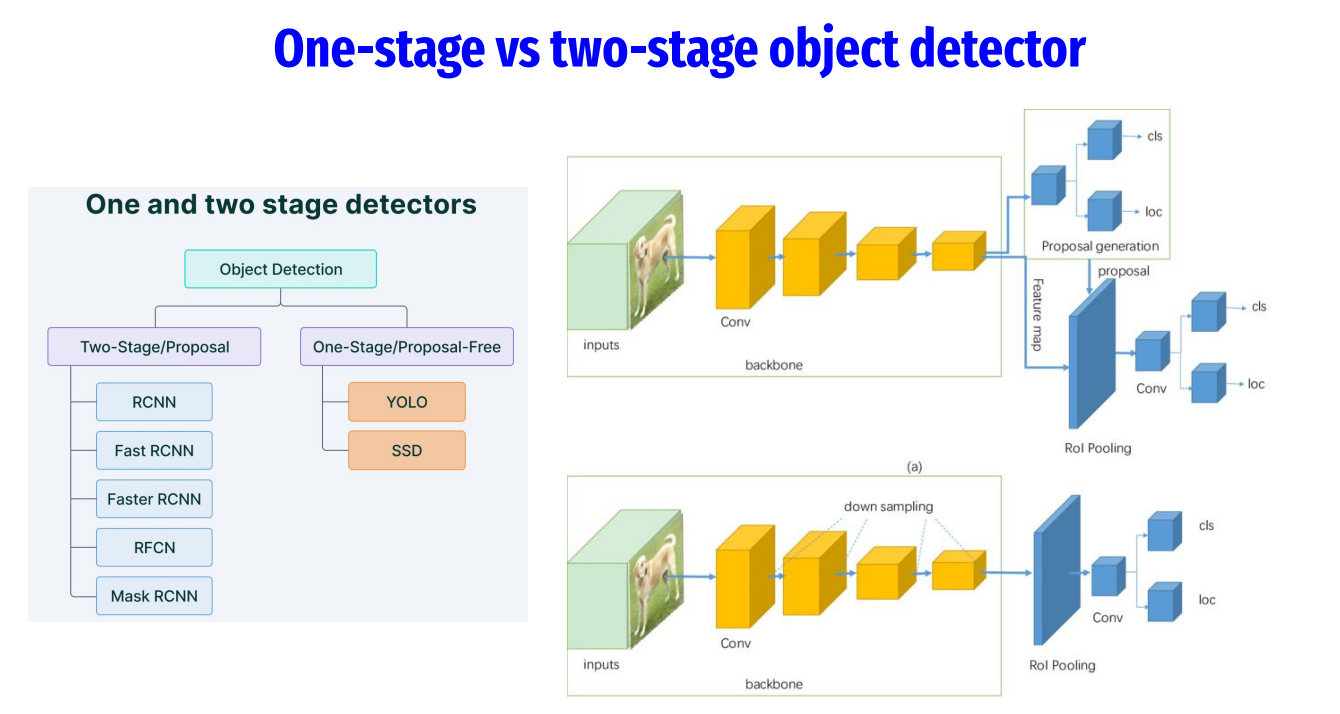
\includegraphics[width=1.28\textwidth]{object_detector.png}
    }
    \caption{Minh họa Single-stage và Two-stage Object Detector}
\end{figure}


\section{Context Modelling:}
\begin{itemize}
    \item[--] Context Modelling là một kỹ thuật để tăng cường khả năng suy luận ngữ cảnh của neurel network, đặc biệt nhằm mục đích phát hiện các khuôn mặt cực kỳ nhỏ (tiny face).
    \item[--] Trong RetinaFace, để tăng cường khả năng capturing tiny faces, SSH \textbf{(Single Stage Headless) - Module for feature extraction} và PyramidBox đã áp dụng context modules trên feature pyramid để mở rộng receptive field từ Euclidean grids.
    \item[--] Để tăng cường non-rigid transformation modelling, RetinaFace sử dụng \textbf{Deformable Convolution Network (DCN)} để thay thế toàn bộ 3 x 3 convolution layers bên trong lateral connections cũng như bên trong chính các context modelling.
\end{itemize}
\section{Multi-task Learning}
\begin{itemize}
    \item[--] Là cách học mà một mô hình có thể giải quyết được nhiều tasks khác nhau
    \item[--] Trong RetinaFace, Multi-task Learning là chiến lược thiết kế một neurel network duy nhất để giải quyết đồng thời nhiều bài toán face detection khác nhau từ cùng một input image, giúp các bài toán chia sẻ feature extraction và bổ trợ chéo cho nhau.
    \item[--] Cấu trúc Multitask-Learning trong RetinaFace: sử dụng một lớp tính toán dùng chung (shared loss head với 1 x 1 convolution layer) áp dụng lên các tầng của feature pyramid. Với mỗi positive anchor, network sẽ dự đoán đồng thời 4 thông tin:
    \begin{itemize}
        \item[+] Face score
        \item[+] Face box 
        \item[+] 5 facial landmarks
        \item[+] Dense 3D face vertices: Cấu trúc 3D dày đặt của khuôn mặt được chiếu lên image plane (self-supervised Learning).  
    \end{itemize}  
    \begin{figure}[H]
        \makebox[\textwidth][c]{
        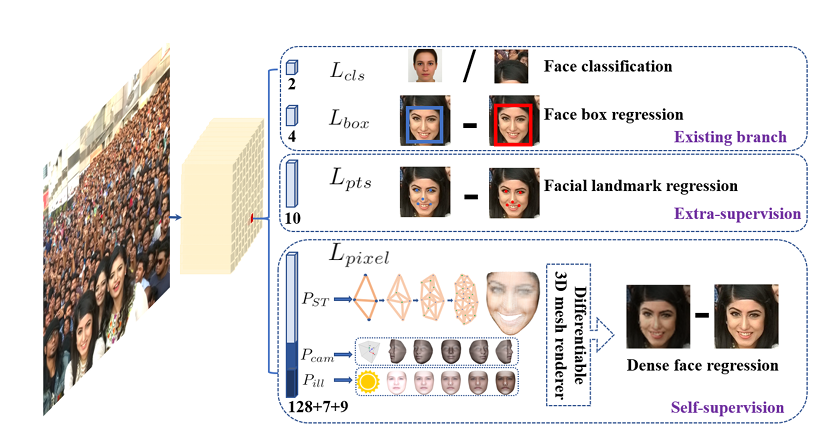
\includegraphics[width=1.20\textwidth]{multitask.png}}
        \caption{Phương pháp single-stage pixel-wise được đề xuất bằng cách sử dụng extra-supervised và self-supervised multi-task learning song song với các box classification và regression branches hiện có. Mỗi positive anchor bao gồm: (1) face score, (2) face box, (3) 5 facial landmarks, (4) dense 3D face vertices được chiếu trên image plane}
    \end{figure}
\end{itemize}
\chapter{RetinaFace Architecture}
\section{Thông tin chung:}
\subsection{Multi-task Loss:}
\begin{itemize}
    \item[--] Với mỗi training anchor \(i\), ta sẽ minimise multi-task loss có công thức:
    \begin{equation}
    L = L_{cls}(p_i,p_i^*) + \lambda_1p_i^*L_{box}(t_i,t_i^*) + \lambda_2p_i^*L_{pts}(l_i,l_i^*) + \lambda_3p_i^*L_{pixel}. \tag{1}
    \end{equation}
    \item[--](1) Face classification loss \(L_{cls}(p_i,p_i^*)\): Là \textbf{Softmax loss for binary classes (face/not face)} dùng để tính xác suất \(p_i\) xem anchor thứ i có phải là face hay không, \(p_i^*\) = 1 nếu positive anchor (có chứa face) và 0 nếu negative anchor
    \item[--](2) Face box regression loss \(L_{box}(t_i,t_i^*)\) Là regression loss:
    \begin{itemize}
        \item[+] Với \(t_i = \{t_x, t_y, t_w, t_h\}_i\) và \(t_i^* = \{t_x^*, t_y^*, t_w^*, t_h^*\}_i\) lần lượt là tọa độ (coordinates) của predicted box và grouth truth box liên quan đến positive anchor \((p_i^* = 1)\)
        \item[+] Paper tuân thủ theo \cite{girshick2015fast} để normalise box regression targets (centre location, width, height) và \(L_{box}(t_i,t_i^*) = R(t_i - t_i^*)\) với \(R\) là robust loss function (smooth-L1) được định nghĩa trong \cite{girshick2015fast}.
    \end{itemize}
    \begin{equation}
    Smooth_{L1}(x) = 
        \begin{cases}
            0.5x^2  & \text{if } |x| < 1 \\ 
            |x| - 0.5 & \text{otherwise,} 
        \end{cases} \tag{1.1}
    \end{equation}
    \item[--](3) Facial landmark regression Loss \(L_{pts}(l_i,l_i^*)\)
    \begin{itemize}
        \item[+] Với \(l_i = \{l_{x_1}, l_{y_1}, \dots, l_{x_5}, l_{y_5}\}_i\) và \(l_i = \{l_{x_1}^*, l_{y_1}^*, \dots, l_{x_5}^*, l_{y_5}^*\}_i\) lần lượt là predicted 5 facial landmarks và grouth truth liên quan đến positive anchor.
        \item[+] Tương tự box centre regression, 5 facial landmark regression cũng sử dụng target normalisation dựa trên anchor centre. 
    \end{itemize}
    \item[--](4) Dense regression loss \(L_{pixel}\) (tham chiếu mục \eqref{eq:pixel_loss})
    \item[--] Loss-balancing parameters \(\lambda_1-\lambda_3\) được gán giá trị lần lượt là 0.25, 0.1 và 0.1. Có nghĩa là ta tăng đáng kể tầm quan trọng của box và landmark locations từ supervision signals.
\end{itemize} 
\subsection{Dense Regression Branch:}
\label{eq:pixel_loss}
\begin{itemize}
    \item [--]\textbf{Mesh Decoder:} paper đã employ trực tiếp mesh decoder (mesh convolution và mesh up-sampling) từ \cite{zhou2019dense,ranjan2018generating}.
    \begin{itemize}
        \item [+] Thay vì sử dụng convolution 2D thông thường (tính toán trên lưới không gian Euclid), nhánh này sử dụng \textbf{Graph Convolution} (tích chập đồ thị) để thao tác với các đỉnh trên mô hình lưới 3D.
        \item [+] Mesh decoder thực hiện dự đoán đồng thời cả shape và texture của face thông qua phương pháp fast localised spectral filtering (lọc phổ quan cục bộ nhanh).
    \begin{figure}[H]
        \makebox[\textwidth][c]{
            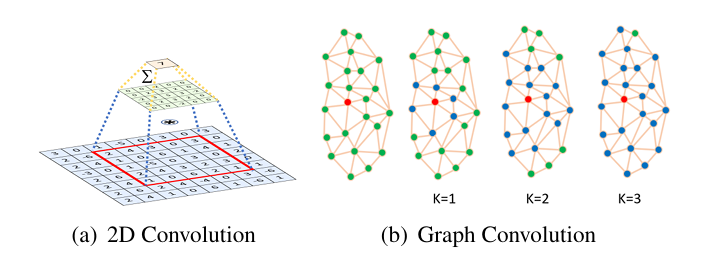
\includegraphics[width=1.0\textwidth]{convolution.png}}
            \caption{Minh họa 2D Convolution trong không gian lưới Euclid và Graph Convolution}
    \end{figure}
    \begin{itemize}
    \item \textbf{(a) 2D Convolution} là một \textit{kernel-weighted neighbour sum} bên trong lưới Euclid receptive field. Mỗi lớp tích chập (\textit{convolutional layer}) chứa \( \text{Kernel}_H \times \text{Kernel}_W \times \text{Channel}_{in} \times \text{Channel}_{out} \) tham số.
    \item \textbf{(b) Graph Convolution} cũng là một dạng của \textit{kernel-weighted neighbour sum}, nhưng khoảng cách lân cận (\textit{neighbour distance}) được tính trên đồ thị bằng cách đếm số cạnh tối thiểu nối giữa hai đỉnh. Mỗi lớp tích chập đồ thị có \( K \times \text{Channel}_{in} \times \text{Channel}_{out} \) tham số và các hệ số Chebyshev \( \theta_{i,j} \in \mathbb{R}^K \) được cắt bớt (\textit{truncated}) ở bậc \( K \).
    \end{itemize}

    \item[+] RetinaFace tuân thủ theo \cite{zhou2019dense} để định nghĩa coloured face mesh \(\mathcal{G} = (\mathcal{V}, \mathcal{E})\), với \(\mathcal{V} \in R^{n \times 6} \) là 1 set của face vertices chưa thông tin về hình dạng (shape) và kết cấu (texture) của khớp (joint), và \(\mathcal{E} \in \{0,1\}^{n \times n}\) là ma trận kề \textbf{thưa} (sparse adjacency matrix) encoding trạng thái kết nối giữa các vertices.
    \item[+] Đồ thị Laplacian được định nghĩa \(\mathcal{L} = \mathcal{D} - \mathcal{E} \in \mathbb{R}^{n \times n}\) với \(\mathcal{D} \in \mathbb{R}^{n \times n}\) là ma trận đường chéo (diagonal matrix) với \(\mathcal{D}_{ii} = \sum_j\mathcal{E}_{ij}\)
    \item[+] Thông qua \cite{zhou2019dense,defferrard2016convolutional,ranjan2018generating}, graph convolution với kernel \(g_\theta\) có thể biểu diễn như recursive Chebyshev polynominal (đa thức Chebyshev đệ quy) được truncated ở bậc K
    \begin{equation}
        y = g_\theta(L)x = \sum_{k=0}^{K-1} \theta_k T_k(\tilde{L})x, \tag{2} 
    \end{equation}
    \item[+] với \(\theta \in \mathbb{R}^K\) là vector của hệ số Chebyshev và \(T_k(\tilde{K} \in \mathbb{R}^{n \times n})\) là đa thức Chebyshev tại bậc k được evaluated tại scale Laplacian \(\tilde{L}\)
    \end{itemize}
\end{itemize}
\begin{equation}
    L_{pixel} = \frac{1}{W * H}\sum_{i}^{W}\sum_{j}^{H} \left\| \mathcal{R}(\mathcal{D}_{P_{ST}}, P_{cam}, P_{ill})_{i,j} - I_{i,j}^* \right\|_1 \tag{3}
\end{equation}

\section{Kiến trúc mô hình RetinaFace:}
\subsection{Backbone:}
\begin{enumerate}
    \item \textbf{MobileNet:}
    \begin{itemize}
        \item abc
    \end{itemize}

    \item \textbf{ResNet:}
    \begin{itemize}
        \item 
    \end{itemize}
\end{enumerate}
\subsection{SSH:}
\subsection{FPN:}

\chapter{RetinaFace Source Code}
\section{Dataset}
\section{Backbone}
\section{Layers}
\section{Loss}
\section{Optimizer}
\section{Model}
\section{Training}
\section{Evaluation}

\chapter{Kết quả và thực nghiệm}
\section{Dataset:}
\section{Implementation details:}
\subsection{Feature Pyramid:}
\subsection{Context Module:}
\subsection{Loss Head:}
\subsection{Data Augmentation:}
\subsection{Training - Testing Details:}
\section{Face box Accuracy}
\section{Five Facial Landmark Accuracy}
\section{Dense Facial Landmark Accuracy}
\section{Face Recognition Accuracy}




\chapter{Kết luận}


\newpage
\bibliographystyle{ieeetr}
\bibliography{tailieu}

\end{document}
